\documentclass[a4paper]{article}
\usepackage[spanish]{babel}
\usepackage[pdftex,usenames,dvipsnames]{color}
\usepackage{multicol}
\usepackage{graphicx}
\usepackage{listings}
\usepackage{color}
\usepackage{hyperref}

\definecolor{dkgreen}{rgb}{0,0.6,0}
\definecolor{gray}{rgb}{0.5,0.5,0.5}
\definecolor{mauve}{rgb}{0.58,0,0.82}

\lstset{
    language=bash, 
    basicstyle=\footnotesize\color{black},
    backgroundcolor=\color{white},
    morekeywords={durar@durar, restart}, keywordstyle=\color{green},
    classoffset=1,
    showspaces=false,
    showstringspaces=false,
    showtabs=false,
    frame=single, 
    tabsize=2,
    captionpos=b,
    breaklines=true,
}
\lstdefinestyle{bashCentOS}{
    language=bash, 
    basicstyle=\footnotesize\color{black},
    backgroundcolor=\color{white},
    morekeywords={durar@localhost, start}, keywordstyle=\color{red},
    classoffset=1,
    showspaces=false,
    showstringspaces=false,
    showtabs=false,
    frame=single, 
    tabsize=2,
    captionpos=b,
    breaklines=true,
}

\begin{document}
\pagestyle{plain}
\title{Práctica 3: Monitorización y "Profiling" \\ 
Ingeniería de Servidores}
\author{Raúl Durán Racero}
\begin{figure}
    \centering
    \includegraphics[width=1.25\textwidth]{servers.pdf}
\end{figure}
\maketitle
\begin{figure}
    \centering
    \includegraphics[width=0.25\textwidth]{logoEtsiit.pdf}
\end{figure}

\newpage
\tableofcontents
\newpage
\section{Ejercicio 1}
Realice una instalación de Zabbix 5.0 en su servidor con \textbf{Ubuntu Server20.04} y configure
para que se monitorice a él mismo y para que monitorice a la máquina con \textbf{CentOS}.
Puede configurar varios parámetros para monitorizar, uso de CPU, memoria, etc. pero
debe configurar de manera obligatoria la monitorización de los servicios \textbf{SSH} y \textbf{HTTP}.
\subsection{Instalación de Zabbix en UbuntuServer}
Por comodidad a la hora de instalar, me conectaré a la máquina virtual de UbuntuServer
a través de SSH, para poder copiar algunos comandos que son muy largos.\newline
Lo primero que tenemos que hacer es instalar Zabbix en Ubuntu. Para ello, 
descargamos su paquete:
\begin{lstlisting}
    durar@durar:~$ wget https://repo.zabbix.com/zabbix/5.0/ubuntu/pool/main/z/zabbix-release/zabbix-release_5.0-1+focal_all.deb
\end{lstlisting}
Una vez descargado, lo instalamos con \textsl{dpkg -i} y obtenemos las actualizaciones
con \textsl{apt update} (es necesario tener permisos de superusuario):
\begin{lstlisting}
    durar@durar:~$ sudo dpkg -i zabbix-release_5.0-1+focal_all.deb
    durar@durar:~$ sudo apt update
\end{lstlisting}
Nos falta instalar el servidor, la interfaz y el agente de Zabbix:
\begin{lstlisting}
    durar@durar:~$ sudo apt install zabbix-server-mysql zabbix-frontend-php zabbix-apache-conf zabbix-agent
\end{lstlisting}
Ya tenemos todo debidamente instalado, por lo que pasaremos a crear una base de 
datos inicial y un usuario, dándole todos los permisos (entraré en mysql como superusuario ya que no 
me permite entrar con \textsl{mysql -u root -p}).
\begin{lstlisting}
    durar@durar:~$ sudo mysql 
    mysql> create database zabbix character set utf8 collate utf8_bin;
    mysql> create user zabbix@localhost identified by 'ISE';
    mysql> grant all privileges on zabbix.* to zabbix@localhost;
    mysql> quit;
\end{lstlisting}
A continuación tenemos que ejectuar el script que establece el esquema por defecto de 
la base de datos.
\begin{lstlisting}
    durar@durar:~$ zcat /usr/share/doc/zabbix-server-mysql*/create.sql.gz | mysql -uzabbix -p zabbix
\end{lstlisting}
Esto puede tardar un tiempo. Podemos comprobar que se está ejecutando con \textsl{htop}
desde la máquina de UbuntuServer:
\begin{figure}
    \centering
    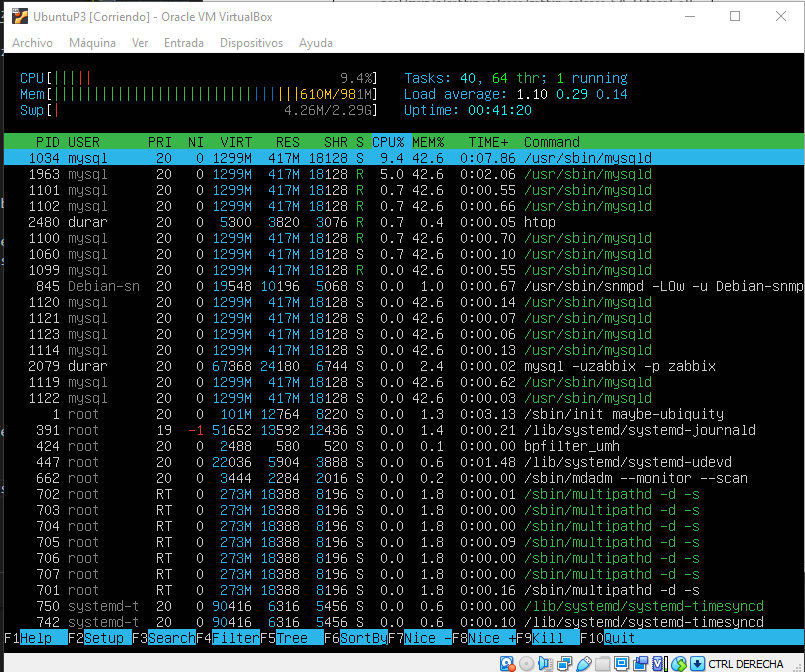
\includegraphics[width=1.0\textwidth]{htop de mysql.png}
\end{figure}
\newpage
Puede verse que efectivamente mysql está en ejecución.\newline
Ya tenemos la base de datos creada, así que ahora toca configurarla.
Primero, editamos el archivo /etc/zabbix/zabbix\_server.conf:
\begin{lstlisting}
    durar@durar:~$ sudo vi /etc/zabbix/zabbix_server.conf
\end{lstlisting}
Y ponemos nuestra contraseña en la línea donde está \textbf{DBPassword}: 
\begin{lstlisting}
    DBPassword=ISE
\end{lstlisting}
Para buscar la línea, se puede usar \textbf{Shift+7} en vi para buscar DBPassword más 
facilmente.\newline
A continuación, configuramos PHP para la interfaz de Zabbix, editando el archivo 
/etc/zabbix/apache.conf, descomentando y cambiando la zona horaria:
\begin{lstlisting}
    durar@durar:~$ sudo vi /etc/zabbix/apache.conf
   > php_value date.timezone Europe/Madrid
\end{lstlisting}
Además de esto, hay que cambiar también el archivo /etc/php/7.4/apache2/php.ini,
ya que si no lo hacemos nos dará un error más tarde, así que lo hacemos ahora:
\begin{lstlisting}
    durar@durar:~$ sudo vi /etc/php/7.4/apache2/php.ini
   > date.timezone = UTC
\end{lstlisting}
Iniciamos los procesos del agente y del servidor de Zabbix y los configuramos
 para que se inicien a la par que el sistema (\textsl{enable}):\newpage
\begin{lstlisting}
    durar@durar:~$ systemctl restart zabbix-server zabbix-agent apache2
    durar@durar:~$ systemctl enable zabbix-server zabbix-agent apache2
\end{lstlisting}
Por último, nos conectamos a nuestra interfaz Zabbix desde el navegador para
instalar el \textsl{frontend: 192.168.56.105/zabbix} \newline
Nos deberá aparecer una interfaz de instalación de Zabbix, donde seguiremos los pasos siguientes:
\begin{description}
    \item[Welcome:] Next Step 
    \item[Check of pre-requisites:] Comprobamos que todo esté correcto -\textgreater Next Step
    \item[Configure DB connection:] Introducimos la contraseña de la BD -\textgreater Next Step   
    \item[Zabbix server details:] Next Step
    \item[Preinstalation summary:] Next Step
    \item[install:] Finish   
\end{description}
Nos notificará de que lo hemos instalado con éxito, y podremos logearnos:
\begin{description}
    \item[User:] Admin
    \item[Password:] zabbix  
\end{description}
\subsection*{Instalación en CentOS}
La instalación en CentOS es similar a la de UbuntuServer, incluso más sencilla, ya que
solo hay que instalar el agente:
Empezamos instalando el repositorio de Zabbix y el paquete del agente:
\begin{lstlisting}[style=bashCentOS]
    [durar@localhost ~]$ sudo rpm -Uvh https://repo.zabbix.com/zabbix/5.0/rhel/8/x86_64/zabbix-release-5.0-1.el8.noarch.rpm
    [durar@localhost ~]$ dnf clean all
    [durar@localhost ~]$ sudo dnf install zabbix-agent
\end{lstlisting}
Hay que cambiar el archivo de configuración en /etc/zabbix/zabbix\_agentd.conf, modificando los valores 
que se muestran resaltados en las siguientes capturas:
\newpage
\begin{figure}
    \centering
    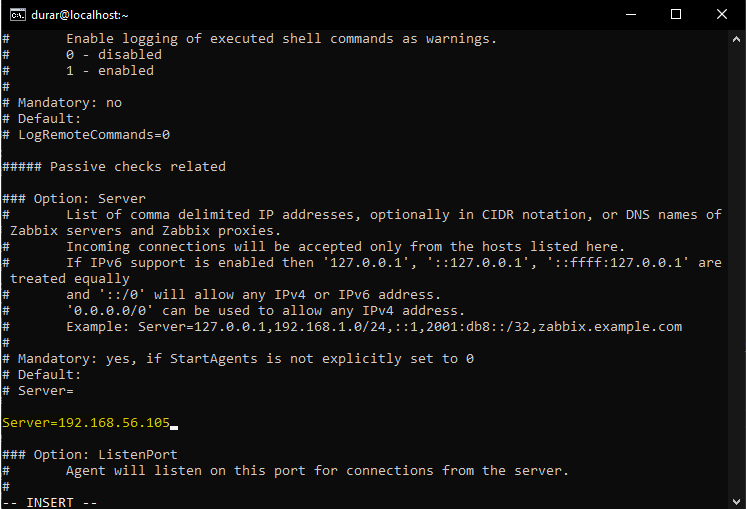
\includegraphics[width=0.8\textwidth]{cambiandoConfZabbigAgent1.png}
    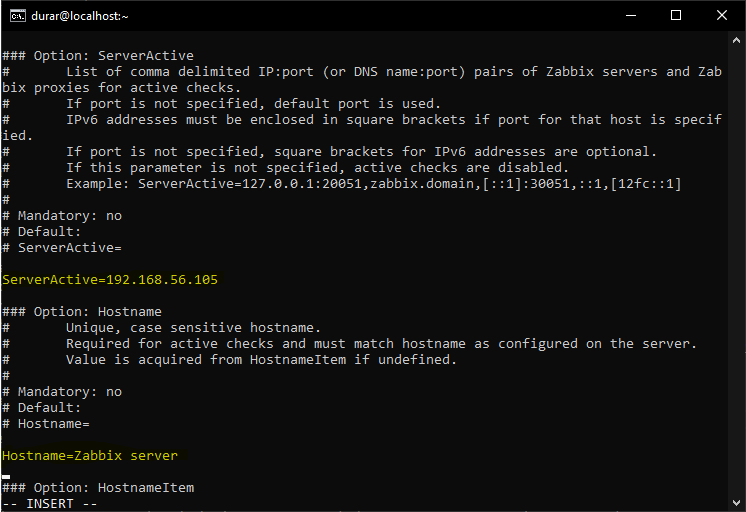
\includegraphics[width=0.8\textwidth]{cambiandoConfZabbigAgent2.png}
\end{figure}
Iniciamos y establecemos el proceso del agente de Zabbix:
\begin{lstlisting}[style=bashCentOS]
    [durar@localhost ~]$ systemctl enable zabbix-agent
    [durar@localhost ~]$ systemctl start zabbix-agent
\end{lstlisting}

\subsection{Configuración}
Ya tenemos el frontend de Zabbix en el navegador, así que ahora añadimos las máquinas que hay que monitorizar.
El host de UbuntuServer viene por defecto con la instalación que hicimos previamente. Este host se encarga 
de monitorizar el propio servidor. Nos falta el de CentOS, así que lo creamos:
Configuration -\textgreater Hosts -\textgreater Create Host y añadir los datos siguientes:
\newpage
\begin{figure}
    \centering
    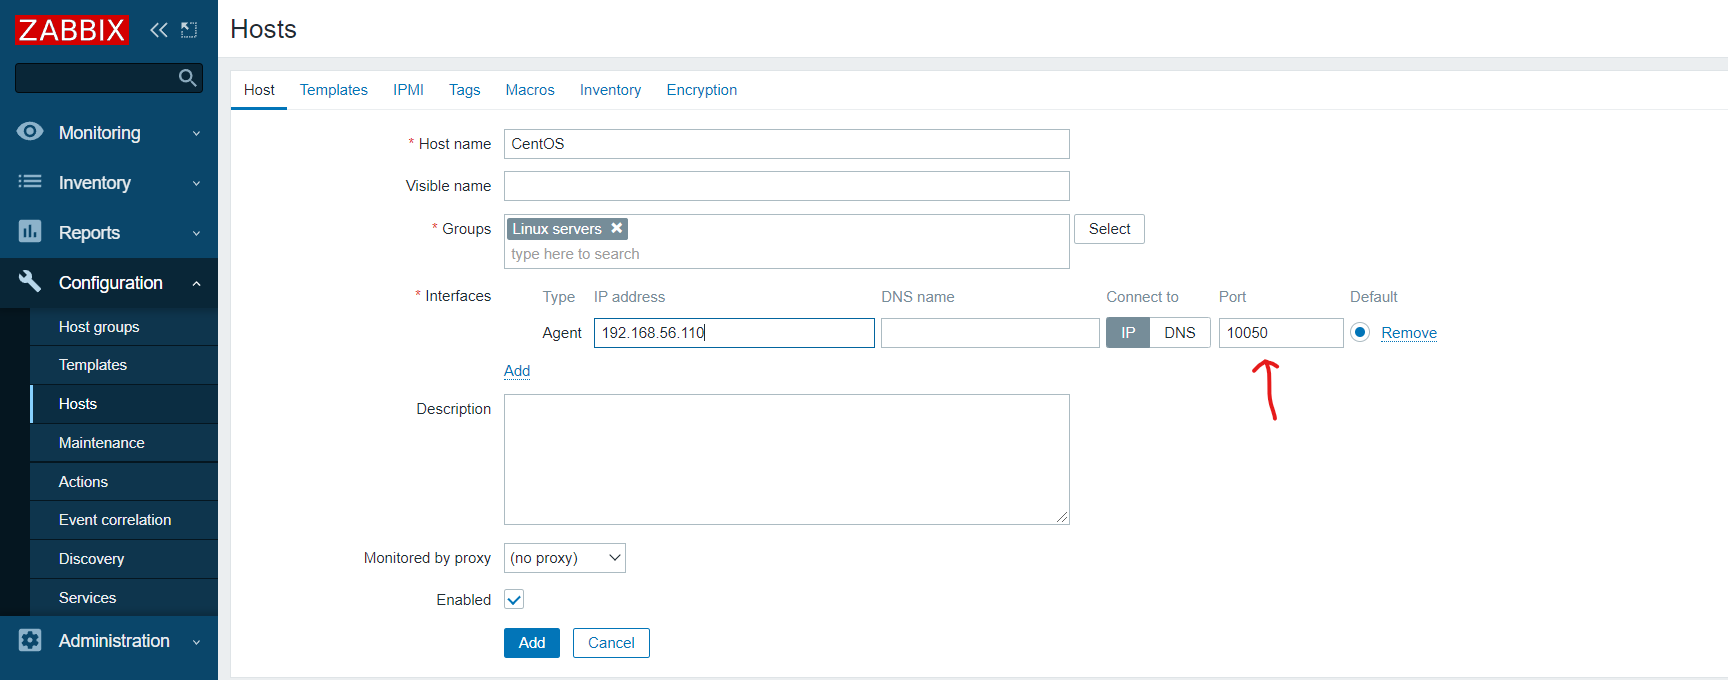
\includegraphics[width=\textwidth]{creando host centos.png}
\end{figure}
Nos daremos cuenta de que el puerto que se utiliza es el 10050, como señala la flecha, así que tendremos 
que abrir dicho puerto en CentOS.
\begin{lstlisting}[style=bashCentOS]
    [durar@localhost ~]$ sudo firewall-cmd --add-port=10050/tcp --permanent
    [durar@localhost ~]$ sudo firewall-cmd --add-port=10050/tcp
    [durar@localhost ~]$ sudo firewall-cmd --reload
\end{lstlisting}
Ya tenemos el puerto abierto y el host de CentOS, así que ya podemos monitorizar ambas máquinas.
Nos piden que monitoricemos los servicios SSH y HTTP en ambas máquinas. Para ello, tenemos que añadir
un nuevo item para cada servicio en las dos máquinas. 
Así que nos dirigimos a Configuration -\textgreater Hosts -\textgreater Zabbix server -\textgreater
Items, le damos a \textsl{Create Item} e introducimos los datos que se muestran en las figuras. Repetimos como 
corresponda para el resto de items.
\newline
\begin{figure}[hbt!]
    \caption{SSH de UbuntuServer}
    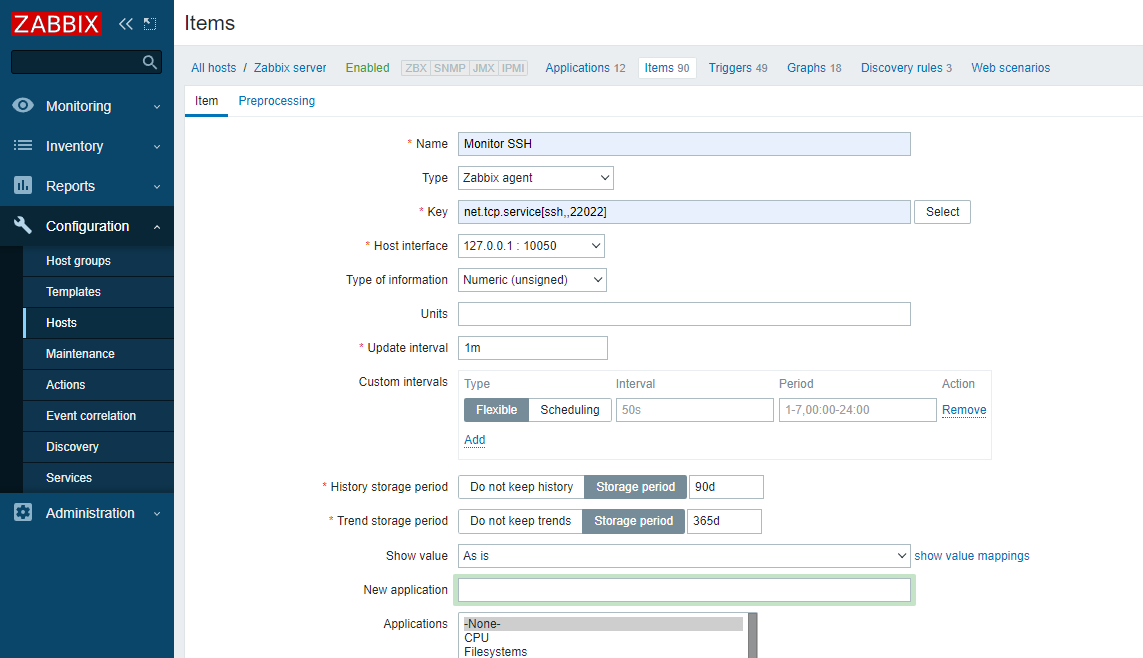
\includegraphics[width=\textwidth]{creando item ssh.png}
\end{figure} 
\newpage
\begin{figure}
    \caption{SSH de CentOS}
    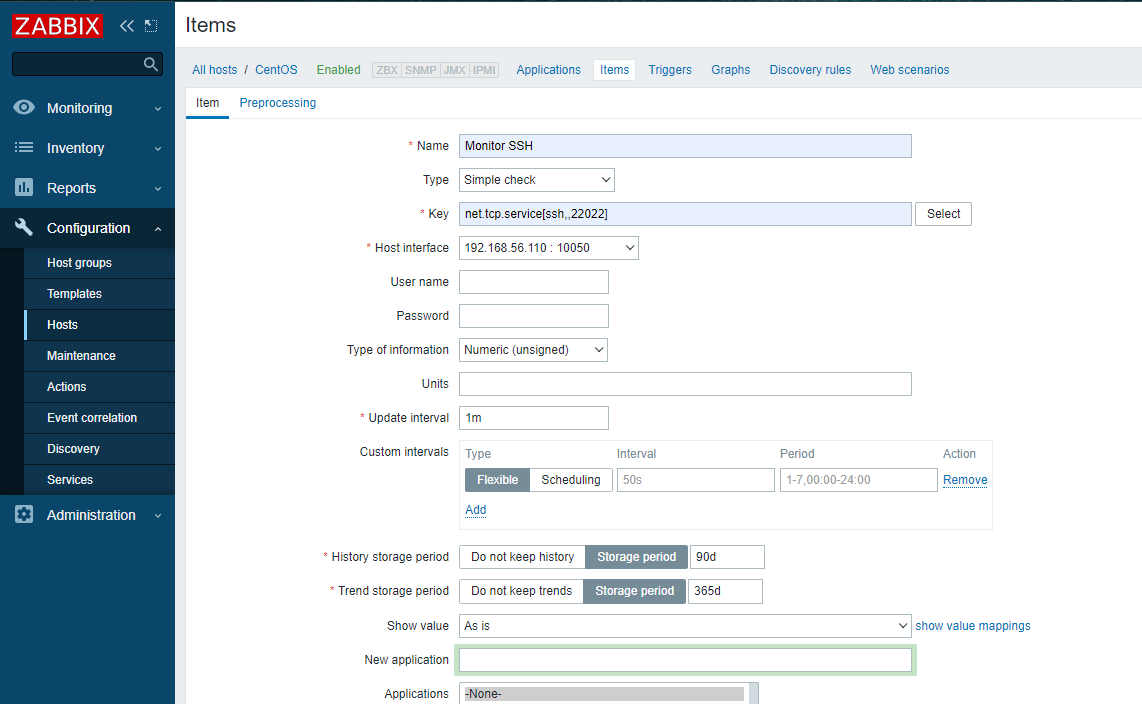
\includegraphics[width=\textwidth]{monitor ssh centos.png}
\end{figure}
Para monitorizar el servicio HTTP en UbuntuServer, queremos comprobar si funciona el servicio de apache.
Zabbix ya nos ofrece un \textsl{Template} configurado para Apache, así que lo utilizaremos:
\begin{figure}[hbt!]
    \caption{HTTP para UbuntuServer}
    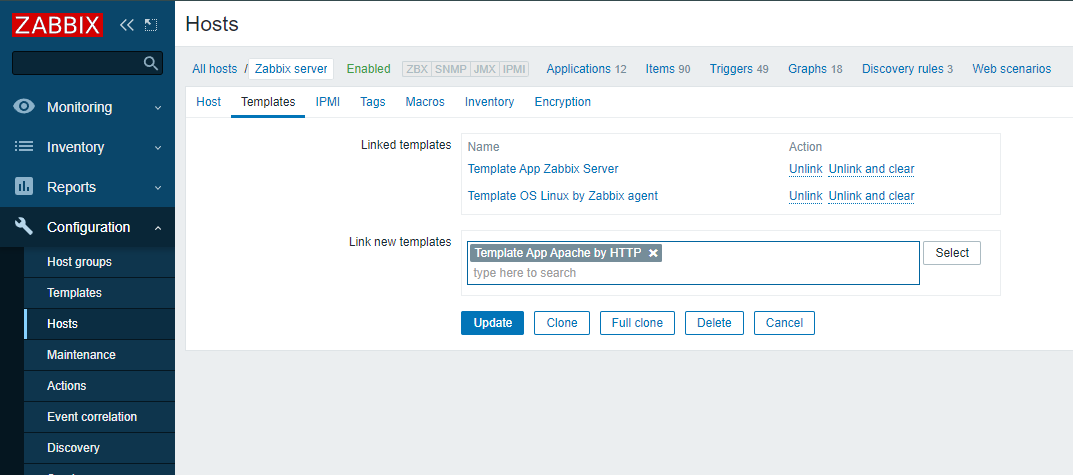
\includegraphics[width=\textwidth]{http para ubunut.png}
\end{figure}
\newpage
\begin{figure}[]
    \caption{HTTP para CentOS}
    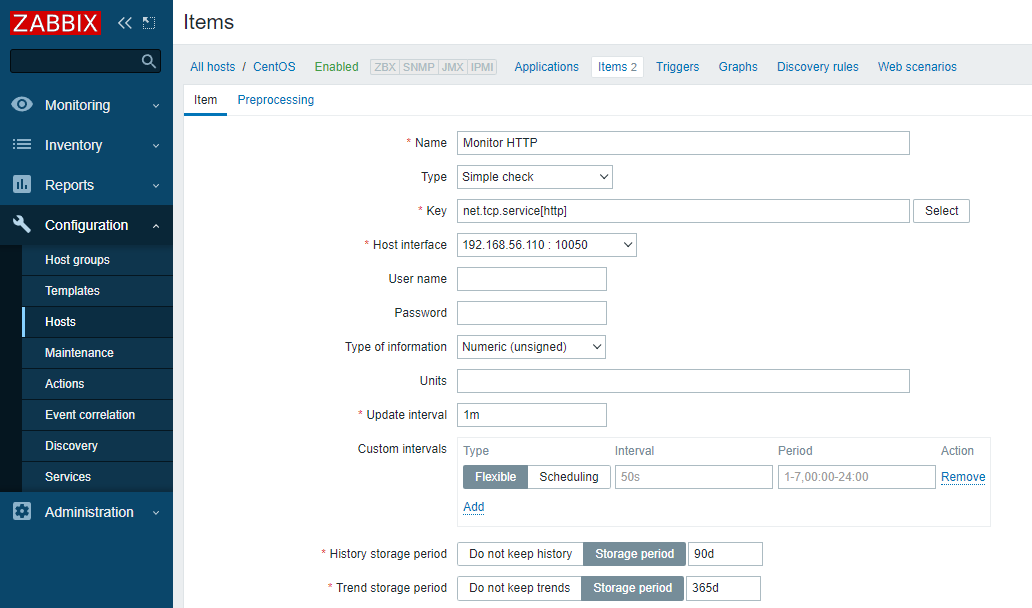
\includegraphics[width=\textwidth]{http centos.png}
\end{figure}
El tipo que hemos escogido en los monitores es \textsl{entering}, ya que lo que queremos es que simplemente
que compruebe si el servicio está activo o no. La \textsl{key} la podemos selectionar en el botón \textsl{Select}.
Además, podemos modificar el intervalo con el que se actualizan los datos monitorizados 
(\textsl{Update Interval}).


\section{Ejercicio 2}
Usted deberá saber cómo instalar y configurar Ansible para poder hacer
un ping a las máquinas virtuales de los servidores y ejecutar un comando básico (p.ej. el
script de monitorización del RAID1). También debe ser consciente de la posibilidad de
escribir acciones más complejas mediante playbooks escritos con YAML.
\newline
Se nos pide instalar y configurar Ansible para poder hacer ping a nuestras máquinas virtuales de 
los servidores, nos hace falta otra máquina que sea la que hace ping. Por eso, clonaremos una de las dos
(en mi caso lo haré en CentOS, por simpleza en la instalación), le cambiaremos su IP para que no 
coincida con la original e instalaremos en ella Ansible. 
Lo primero será, una vez clonada la máquina, cambiar su IP como hicimos en la práctica 1:
\begin{lstlisting}[style=bashCentOS]
    [durar@localhost ~]$ sudo vi /etc/sysconfig/network-scripts/ifcfg-enp0s8
\end{lstlisting}
La Ip de la nueva máquina será \textbf{192.168.56.111}. Reiniciamos para aplicar los cambios y
comprobamos la IP con \textsl{ifconfig}.
Ahora toca instalar Ansible:
\begin{lstlisting}[style=bashCentOS]
    [durar@localhost ~]$ sudo yum install epel-release
    [durar@localhost ~]$ sudo yum install ansible
\end{lstlisting}
Una vez, instalado, lo coniguramos editando el archivo /etc/ansible/hosts y añadimos las IPs de nuestras
máquinas, con el puerto 22022, junto a una etiqueta que forme el grupo.
\newpage
\begin{figure}
    \centering
    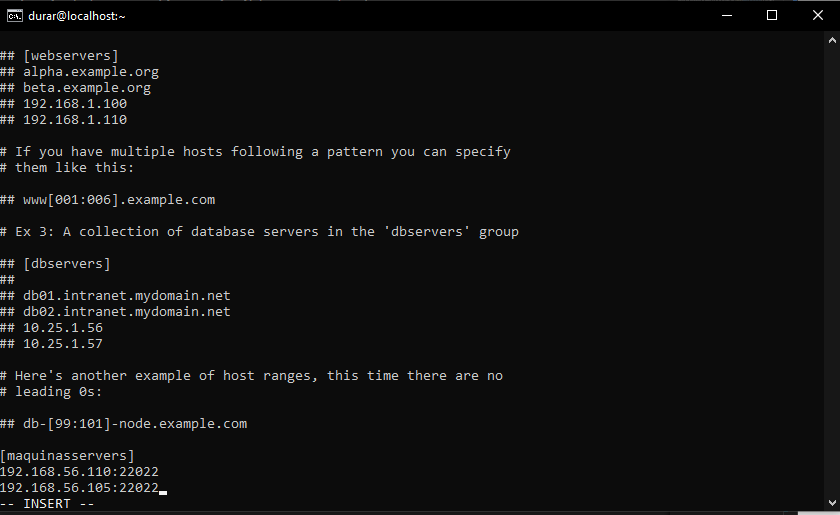
\includegraphics[width=\textwidth]{cambiando conf de ansible1.png}
\end{figure}
Ansible se comunica con las máquinas remotas mediante el protocolo SSH, así que al igual que en la 
práctica anterior, crearemos y añadiremos la clave pública a las máquinas:
\begin{lstlisting}[style=bashCentOS]
    [durar@localhost ~]$ ssh-keygen
    [durar@localhost ~]$ ssh-copy-id 192.168.56.110 -p 22022
    [durar@localhost ~]$ ssh-copy-id 192.168.56.105 -p 22022
\end{lstlisting}
Comprobamos con ssh que se han copiado bien, y hacemos ping:
\begin{lstlisting}[style=bashCentOS]
    [durar@localhost ~]$ ansible -m ping "maquinasservers"
\end{lstlisting}
Nos dará una salida como esta:
\begin{figure}[hbt!]
    \centering
    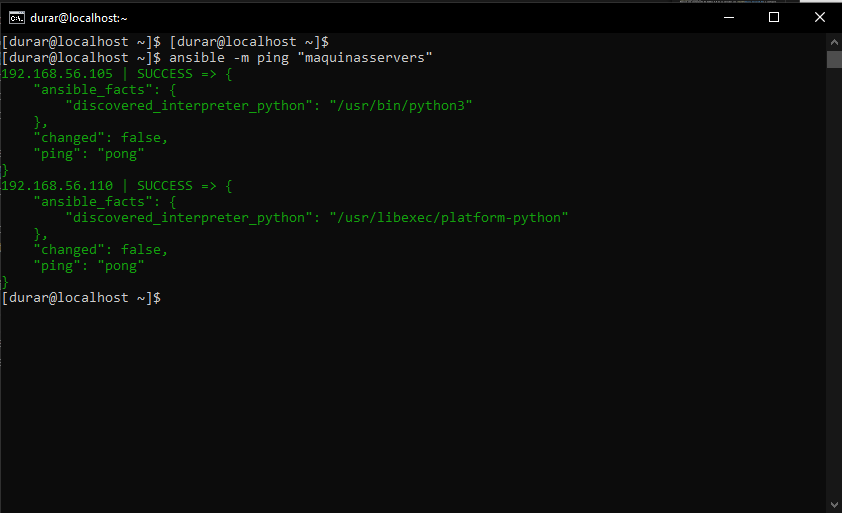
\includegraphics[width=\textwidth]{salida de ansible ping.png}
\end{figure}
\newline También podemos ejecutar el script de monitorización del RAID1 que vimos en clase:
\begin{lstlisting}[style=bashCentOS]
    [durar@localhost ~]$ ansible "maquinasservers" -a "python3 mon_raid.py"
\end{lstlisting}
Ansible nos permite escribir acciones más complejas mediante unos documentos YAML, los \textsl{playbooks}.
Crearemos uno que cree un archivo temporal y nos muestre el estado del servicio SSH:
\begin{figure}[hbt!]
    \centering
    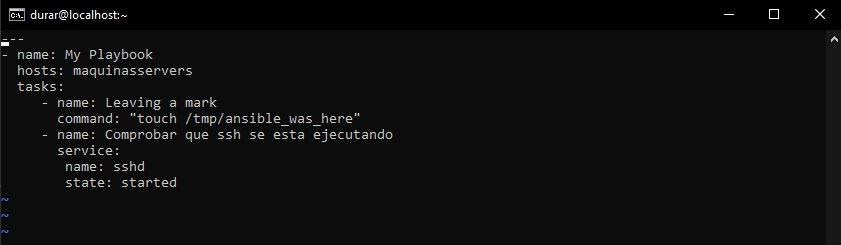
\includegraphics[width=\textwidth]{mi playbook.png}
\end{figure}
\newline Para ejecutarlo:
\begin{lstlisting}[style=bashCentOS]
    [durar@localhost ~]$ ansible-playbook myplaybook.yaml
\end{lstlisting}
Nos dará la siguiente salida:
\begin{figure}[hbt!]
    \centering
    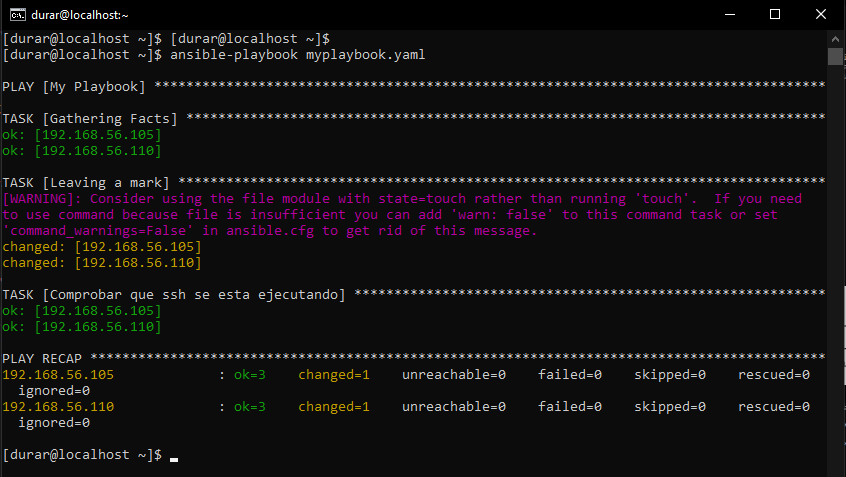
\includegraphics[width=\textwidth]{salida de playbook.png}
\end{figure}
\newline Vemos que nos muestra un warning por el touch, y nos dice como solucionarlo o ignorarlo, pero 
acepta la otra tarea, que se ejecuta correctamente.
\newpage
\begin{thebibliography}{99}
    \bibitem[Zabbix Ubuntu]{instalar zabbix en ubuntu} 
    \href{https://www.zabbix.com/la/download?zabbix=5.0&os_distribution=ubuntu&os_version=20.04_focal&db=mysql&ws=apache}{Instalar y configurar Zabbix en Ubuntu}
    \bibitem[Zabbix CentOS]{instalar zabbix en CentOS} 
    \href{https://www.zabbix.com/la/download?zabbix=5.0&os_distribution=centos&os_version=8&db=mysql&ws=apache}{Instalar y configurar Zabbix en CentOS}
    \bibitem[Configurar frontend Zabbix]{frontend zabbix}
    \href{https://www.zabbix.com/documentation/5.0/manual/config}{Configurar hosts e items de Zabbix} 
    \bibitem[Instalar Ansible]{instalar ansible}
    \href{https://docs.ansible.com/ansible/latest/installation_guide/intro_installation.html#installing-ansible-on-rhel-centos-or-fedora}{Instalar Ansible en CentOS} 
    \bibitem[Empezar en Ansible]{empezar ansible}
    \href{https://docs.ansible.com/ansible/latest/user_guide/index.html#getting-started}{Guión de como empezar en ansible, y escribir tareas y playbooks}
\end{thebibliography}
\end{document}